\documentclass[xetex,mathserif,serif,10pt]{beamer}
%\documentclass[xetex,mathserif,serif,10pt,handout]{beamer}

\usepackage{fontspec}
\usepackage{xunicode}
\usepackage{xltxtra}
\usepackage{graphicx}
\usepackage{bm}
\usepackage{comment}
\usepackage{multicol}
\usepackage[absolute,overlay,quiet]{textpos}
\usepackage{commath}
\usepackage{etaremune}
\usepackage{wasysym}

\defaultfontfeatures{Mapping=tex-text}
\setmainfont{Linux Libertine O}
\chardef\&="E050

\usepackage[margin=10pt,font=small,labelfont=bf,textfont=it,labelsep=colon,singlelinecheck=false,justification=justified]{caption}
\usepackage[spanish]{babel}
\usepackage[final,expansion=true,protrusion=true,spacing=true,kerning=true]{microtype}

\mode<presentation> {
  %\hypersetup{pdfpagemode=FullScreen} %para poner en modo fullscreen de una
  \usetheme{Boadilla} % Pretty neat, soft color.
  \usecolortheme{orchid}
  \definecolor{chart00}{rgb}{0.00,0.00,0.00}
  \definecolor{chart01}{rgb}{0.00,0.27,0.53}
  \definecolor{chart02}{rgb}{1.00,0.26,0.05}
  \definecolor{chart03}{rgb}{1.00,0.83,0.13}
  \definecolor{chart04}{rgb}{0.34,0.62,0.11}
  \definecolor{chart05}{rgb}{0.49,0.00,0.13}
  \definecolor{chart06}{rgb}{0.51,1.15,1.00}
  \definecolor{chart07}{rgb}{0.19,0.25,0.02}
  \definecolor{chart08}{rgb}{0.68,0.81,0.00}
  \definecolor{chart09}{rgb}{0.29,0.12,0.44}
  \definecolor{chart10}{rgb}{1.00,0.58,0.05}
  \definecolor{chart11}{rgb}{0.77,0.00,0.04}
  \definecolor{chart12}{rgb}{0.00,0.52,0.82}
  \definecolor{chart13}{rgb}{1.00,1.00,1.00}
  \definecolor{beamer@blendedblue}{rgb}{0.,0.27,0.53}

  \setbeamercolor{normal text}{fg=black}
  \setbeamercolor{alerted text}{fg=chart11}
  \setbeamercolor{example text}{fg=chart08}
  %\setbeamercovered{transparent}%transparencia en las pausas
  %\beamertemplatetransparentcovereddynamicmedium
  %\setbeamertemplate{navigation symbols}{}
  \setbeamercolor{author}{fg=chart05}
  \AtBeginSection[]
  {
    \begin{frame}
      \frametitle{Contenidos}
      \tableofcontents[currentsection]
    \end{frame}
  }
}

\logo{
\includegraphics[height=1.5cm]{logo-uis.png}}
\newcommand{\bblock}[1]{{\color{chart12}{#1}}}
\newcommand{\bc}[1]{
  \begin{center}
  #1
  \end{center}
}
\newcommand{\be}[2]{
  \vspace{-0.5em}
  \begin{equation}\label{#2}
    #1
  \end{equation}
  \vspace{-1em}
}

\def \unidad 	  {01}
\def \clase 	  {04}
\def \contenido {Probabilidades}
\def \contone	  {probabilistica}
\def \fecha 	  {20130913}
\def \dia	      {V}
\def \autor     {HA}
\def \file	{\unidad-\clase-\fecha\dia-\autor-\contone.pdf}

\title[\contone]{Introducción a la Física de Partículas\\\vspace*{1cm}\unidad-\clase\\\contenido}
\author[H. Asorey]{\Large{Hernán Asorey}}
\institute[hasorey@uis.edu.co]{
	Escuela de Física, Universidad Industrial de Santander\\
	Bucaramanga, Colombia\\
	\color{chart09}{\large{hasorey@uis.edu.co}}\\
	\color{chart05}{\large{\fecha\dia}}
}
\date[\fecha\dia]{\color{chart07}{\file}}

\begin{document}
%\tikzstyle{every picture}+=[remember picture]
%\everymath{\displaystyle}

\begin{comment}
\end{comment}
%%%%%%%%%%%%%%%%%%%%%%%
\begin{frame}
\titlepage
\end{frame}

\logo{}

% \begin{textblock*}{22mm}(100mm,0.25\textheight)
% \begin{exampleblock}
% \tiny{Kotera et al, ARAA49:119(2011)53}
% \end{exampleblock}
% \end{textblock*}
% \begin{textblock*}{35mm}(90mm,0.00\textheight)
% 	\begin{alertblock}{Posibles fuentes}
% 		\begin{itemize}
% 			\item AGN
% 			\item Magnetars
% 			\item GRBs
% 		\end{itemize}
% 	\end{alertblock}
% \end{textblock*}

%%%%%%%%%%%%%%%%%%%%%%%%%%%%%%%%%%%%%%%%%%%
\section{Repaso clase anterior}
%%%%%%%%%%%%%%%%%%%%%%%%%%%%%%%%%%%%%%%%%%%

\begin{frame}
  \frametitle{Boosts}
  \begin{itemize}
    \item Transformaciones de Lorentz no rotantes: {\emph{cambios entre marcos de referencia incerciales}}
    \item Quedan definidos por el $\gamma$ de Lorentz (estrictamente $\beta \to \mathbf{\beta}=\mathbf{v}/c$)
    \item Y luego, $S \to S'$
    \begin{equation}\label{EQboost}
      \left (
        \begin{array}{c}
          t' \\
          x' \\
          y' \\
          z' \\
        \end{array}
      \right ) 
      = 
      \left (
        \begin{array}{cccc}
          \gamma & -\beta\gamma & 0 & 0 \\
          -\beta\gamma & \gamma & 0 & 0 \\
          0 & 0 & 1 & 0 \\
          0 & 0 & 0 & 1
        \end{array}
      \right )
      \left (
        \begin{array}{c}
          t \\
          x \\
          y \\
          z \\
        \end{array}
      \right ) 
    \end{equation}
  \item o en general, para un boost a un sistema con velocidad $\mathbf{v}=(\beta_1, \beta_2, \beta_3) c$, la TL se puede expresar mediante una matriz de $4\times4$, $\Lambda\equiv\Lambda_{ij}$, donde,
    \begin{eqnarray*}
      \Lambda_{00} &=& \gamma,\\
      \Lambda_{i0}=\Lambda_{0i} &=& -\beta_i \gamma,\\
      \Lambda_{ij}=\Lambda_{ji} &=& \delta_{ij} + (\gamma - 1) \frac{\beta_i \beta_j}{\beta^2}.
    \end{eqnarray*}
  \end{itemize}
\end{frame}

\begin{frame}
	\frametitle{Cálculo Tensorial}
  \framesubtitle{Caldo Knorr\textregistered:~ Hernández\& Núñez, ``Métodos de Matemáticas Aplicadas'', Vol 1, Cap 3}
  \begin{itemize}
    \item Convención de Einstein en notación covariante: $\sum_{\mu=0}^3 x_\mu x^\mu \equiv x_\mu x^\mu$
    \item Índices latinos, $i,j,k,\ldots$: componentes espaciales ($1\ldots 3$),
    \item Índices griegos $\mu, \nu, \rho, \ldots$: espaciotemporales ($0\ldots 3$)
    \item Métrica de Minkowsky (plana), convención de signos usual en partículas, $\eta=(1,-1,-1,-1)$.
    \item El tensor métrico $g_{\mu\nu}$ queda entonces:
      \begin{equation}\label{EQmetrica}
        \mathbf{g} \equiv g_{\mu\nu} = \left ( 
          \begin{array}{cccc}
            1 & 0 & 0 & 0 \\
            0 & -1 & 0 & 0 \\
            0 & 0 & -1 & 0 \\
            0 & 0 & 0 & -1
          \end{array}
          \right ) = g^{\mu\nu}\equiv \mathbf{g}^{-1}
      \end{equation}
    \item Definimos {\bf{cuadrivector contravariante}} (cuadrivector) a un \alert{tensor contravariante de rango $1$}, que ante una transformación de Lorentz Λ se comporta como:
      \begin{equation}
        a'^\mu = \Lambda^{\mu}_{\nu} a^\nu
      \end{equation}
  \end{itemize}
  \begin{textblock*}{41mm}(84mm,0.38\textheight)
    \tiny 
    {
      \begin{exampleblock}{\tiny{Tarea (cont)}}
        \begin{enumerate}\setcounter{enumi}{04}
          \item Verficar que $\mathbf{g}\mathbf{g}^{-1} = g_{\nu\rho} g^{\mu\rho} = \delta^\mu_\nu$
          \item Verificar la relación de pseudo-ortogonalidad de las TL: \vspace{-2em}  
           \begin{equation}\label{EQorto}
             g_{\mu\nu} \Lambda^{\mu}_{\rho} \Lambda^{\nu}_{\sigma} = g_{\rho\sigma}
           \end{equation}\vspace{-3em}  
        \end{enumerate}
      \end{exampleblock}
    }
  \end{textblock*}
  \begin{textblock*}{41mm}(84mm,0.89\textheight)
    \Large{\alert{\bf{Cuadrivector}}}
  \end{textblock*}
\end{frame}

\begin{frame}
	\frametitle{cos y contras}
  \begin{itemize}
    \item Cada vector contravariante (vector) tiene asociado un vector covariante (forma), gracias a la métrica (contra $\to$ co)
      \begin{equation}
         (t,-\mathbf{r}) = a_\mu = g_{\mu\nu} a^\nu
      \end{equation}
    \item La transformación inversa co$\to$contra:
      \begin{equation}
        (t,\mathbf{r}) = a^\mu = g^{\mu\nu} a_\nu
      \end{equation}
    \item ¿Cómo transforma un vector covariante frente a una TL $\Lambda$?\\
      \begin{columns}
        \column{0.10\textwidth}
        \column{0.40\textwidth}
        \begin{eqnarray}
          a'_\mu &=& g_{\mu\nu} a'^\nu \nonumber\\ 
          a'_\mu &=& g_{\mu\nu} \Lambda^{\nu}_{\rho} a^\rho \nonumber\\
          a'_\mu &=& \underbrace{g_{\mu\nu} \Lambda^{\nu}_{\rho} g^{\rho\sigma}}_{\left ( \Lambda^{-1} \right )^\sigma_\mu} a_\sigma \nonumber
        \end{eqnarray}
        \vspace{-2em}
        \begin{alertblock}{}
          \begin{equation}
            a'_\mu = \left ( \Lambda^{-1} \right )^\sigma_\mu a_\sigma
          \end{equation}
        \end{alertblock}
        {\small{Queremos probar que el factor $g_{\mu\nu} \Lambda^{\nu}_{\rho} g^{\rho\sigma}$ es la TL inversa.}}
        \column{0.50\textwidth}
        {\small{Entonces recordamos (\ref{EQmetrica}) y (\ref{EQorto}):}}
        \begin{eqnarray}
          g_{\rho\theta} &=& g_{\mu\nu} \Lambda^{\nu}_{\rho} \Lambda^{\mu}_{\theta} \nonumber\\
          g_{\rho\theta} g^{\rho\sigma} &=& g_{\mu\nu} \Lambda^{\nu}_{\rho} \Lambda^{\mu}_{\theta}  g^{\rho\sigma} \nonumber \\
          \delta^{\sigma}_{\theta} &=& \underbrace{\left ( g_{\mu\nu} \Lambda^{\nu}_{\rho}  g^{\rho\sigma} \right )}_{\Xi^\sigma_\mu} \Lambda^{\mu}_{\theta} \nonumber \\
          \delta^{\sigma}_{\theta}  &=& \Xi_\mu^\sigma \Lambda^{\mu}_{\theta} \to \Xi_\mu^\sigma \left (\Lambda^{-1} \right )^\sigma_\mu \nonumber
        \end{eqnarray}
        \vspace{-2.0em}
        \begin{exampleblock}{}
          \begin{equation}
            \Rightarrow \left (\Lambda^{-1} \right )^\sigma_\mu = g_{\mu\nu} \Lambda^{\nu}_{\rho} g^{\rho\sigma}
          \end{equation}
        \end{exampleblock}
      \end{columns}
  \end{itemize}
  \begin{textblock*}{30mm}(6mm,0.70\textheight)
    \small{\alert{Si $\Lambda$ es un boost $\beta$, $\Lambda^{-1}$ es un boost $-\beta$}}
  \end{textblock*}
\end{frame}

\begin{frame}
  \frametitle{\alert{Tarea 03 (último)}}
  \begin{enumerate}\setcounter{enumi}{04}
    \item Verificar explicitamente que $p^\mu p_\mu$ es un invariante ante TL
    \item Griffiths: leer sección 3.4, para discutir en clase 04
    \item Griffiths: problemas 3.4, 3.11, 3.12, 3.14, y alguno del 3.15
  \end{enumerate}
\end{frame}

%%%%%%%%%%%%%%%%%%%%%%%%%%%%%%%%%%%%%%%%%%%
\section{Cálculo Tensorial}
%%%%%%%%%%%%%%%%%%%%%%%%%%%%%%%%%%%%%%%%%%%

\begin{frame}
\frametitle{(covariantes $\cdot$ contravariantes) $\to$ invariantes}
  \begin{itemize}
    \item Propuesta 1: \alert{La composición de dos TL es una TL}:
      \begin{eqnarray}
        a'^\mu &=& \Lambda^{\mu}_{\nu} a^\nu \qquad \mathrm{y} \qquad a''^\rho = \Lambda'^{\rho}_{\mu} a'^\mu \nonumber\\
        \to a''^\rho &=& \Lambda'^{\rho}_{\mu} \Lambda^{\mu}_{\nu} a^\nu \nonumber\\
        a''^\rho &=& \left (\Lambda' \Lambda \right)^{\rho}_{\nu} a^\nu \nonumber\\
        a''^\rho &=& \Lambda''^{\rho}_{\nu} a^\nu
      \end{eqnarray}
    \item Propuesta 2: \alert{El producto escalar $\mathbf{a}\cdot\mathbf{b}\equiv a_\mu b^\nu = a^\mu b_\nu$ es invariante ante transformaciones de Lorentz}:
      \begin{eqnarray}
        \mathbf{a'} \cdot \mathbf{b'} &=& a'_\mu b'^\mu \nonumber\\
        \mathbf{a'} \cdot \mathbf{b'} &=& (\Lambda^{-1})_\mu^\sigma a_\sigma \Lambda_\rho^\mu b^\rho \nonumber\\
        \mathbf{a'} \cdot \mathbf{b'} &=& (\Lambda^{-1})_\mu^\sigma \Lambda_\rho^\mu a_\sigma  b^\rho \nonumber\\
        \mathbf{a'} \cdot \mathbf{b'} &=& \delta^\sigma_\rho a_\sigma b^\rho \nonumber\\
        \mathbf{a'} \cdot \mathbf{b'} &=& a_\rho b^\rho = \mathbf{a} \cdot \mathbf{b}
      \end{eqnarray}
  \end{itemize}
\end{frame}

\begin{frame}
  \frametitle{Tres invariantes famosos tres}
  \begin{itemize}
    \item \alert{Invariante $ds^2$}:
      \begin{equation}
        ds^2 \equiv dx^\mu dx_\mu = d(ct)^2 - (dx)^2 - (dy)^2 - (dz)^2
      \end{equation}
    \item \alert{Derivadas parciales}:
      \begin{equation}
        \frac{\partial}{\partial^\mu} \equiv \partial_\mu = \left( \frac{\partial}{\partial t}, \nabla \right)
        \qquad \mathrm{y} \qquad
        \frac{\partial}{\partial_\mu} \equiv \partial^\mu = g^{\mu\nu} \partial_\nu = \left(\frac{\partial}{\partial t}, -\nabla \right)
      \end{equation}
      y luego, el invariante es el operador \alert{D'alambertiano}:
      \begin{equation}
        \partial_\mu \partial^\mu = \left(\frac{\partial^2}{\partial t^2} - \nabla^2 \right) \equiv \square
      \end{equation}
    \item \alert{Cuadrivector Energía-momento}: Recordando clase 01-01: $E=\gamma m_0$ y $\mathbf{p}=\gamma m_0 \mathbf{v}$, podemos formar un cuadrivector:
      \begin{equation}
        p^\mu \equiv (E,\mathbf{p}) \qquad \mathrm{y} \qquad  p_\mu = g_{\mu\nu} p^\nu \equiv (E,-\mathbf{p})
      \end{equation}
      y luego, contrayendo, obtenemos uno de los invariantes más importantes:
      \begin{alertblock}{
          \begin{equation}
            p^\mu p_\mu \equiv p^2 = E^2 -\mathbf{p}^2 = m_0^2
          \end{equation}
      }
    \end{alertblock}
  \end{itemize}
\end{frame}

%%%%%%%%%%%%%%%%%%%%%%%%%%%%%%%%%%%%%%%%%%%
\section{Probabilística y Colisional}
%%%%%%%%%%%%%%%%%%%%%%%%%%%%%%%%%%%%%%%%%%%

\begin{frame}
  \frametitle{Colisiones}
  {\centering 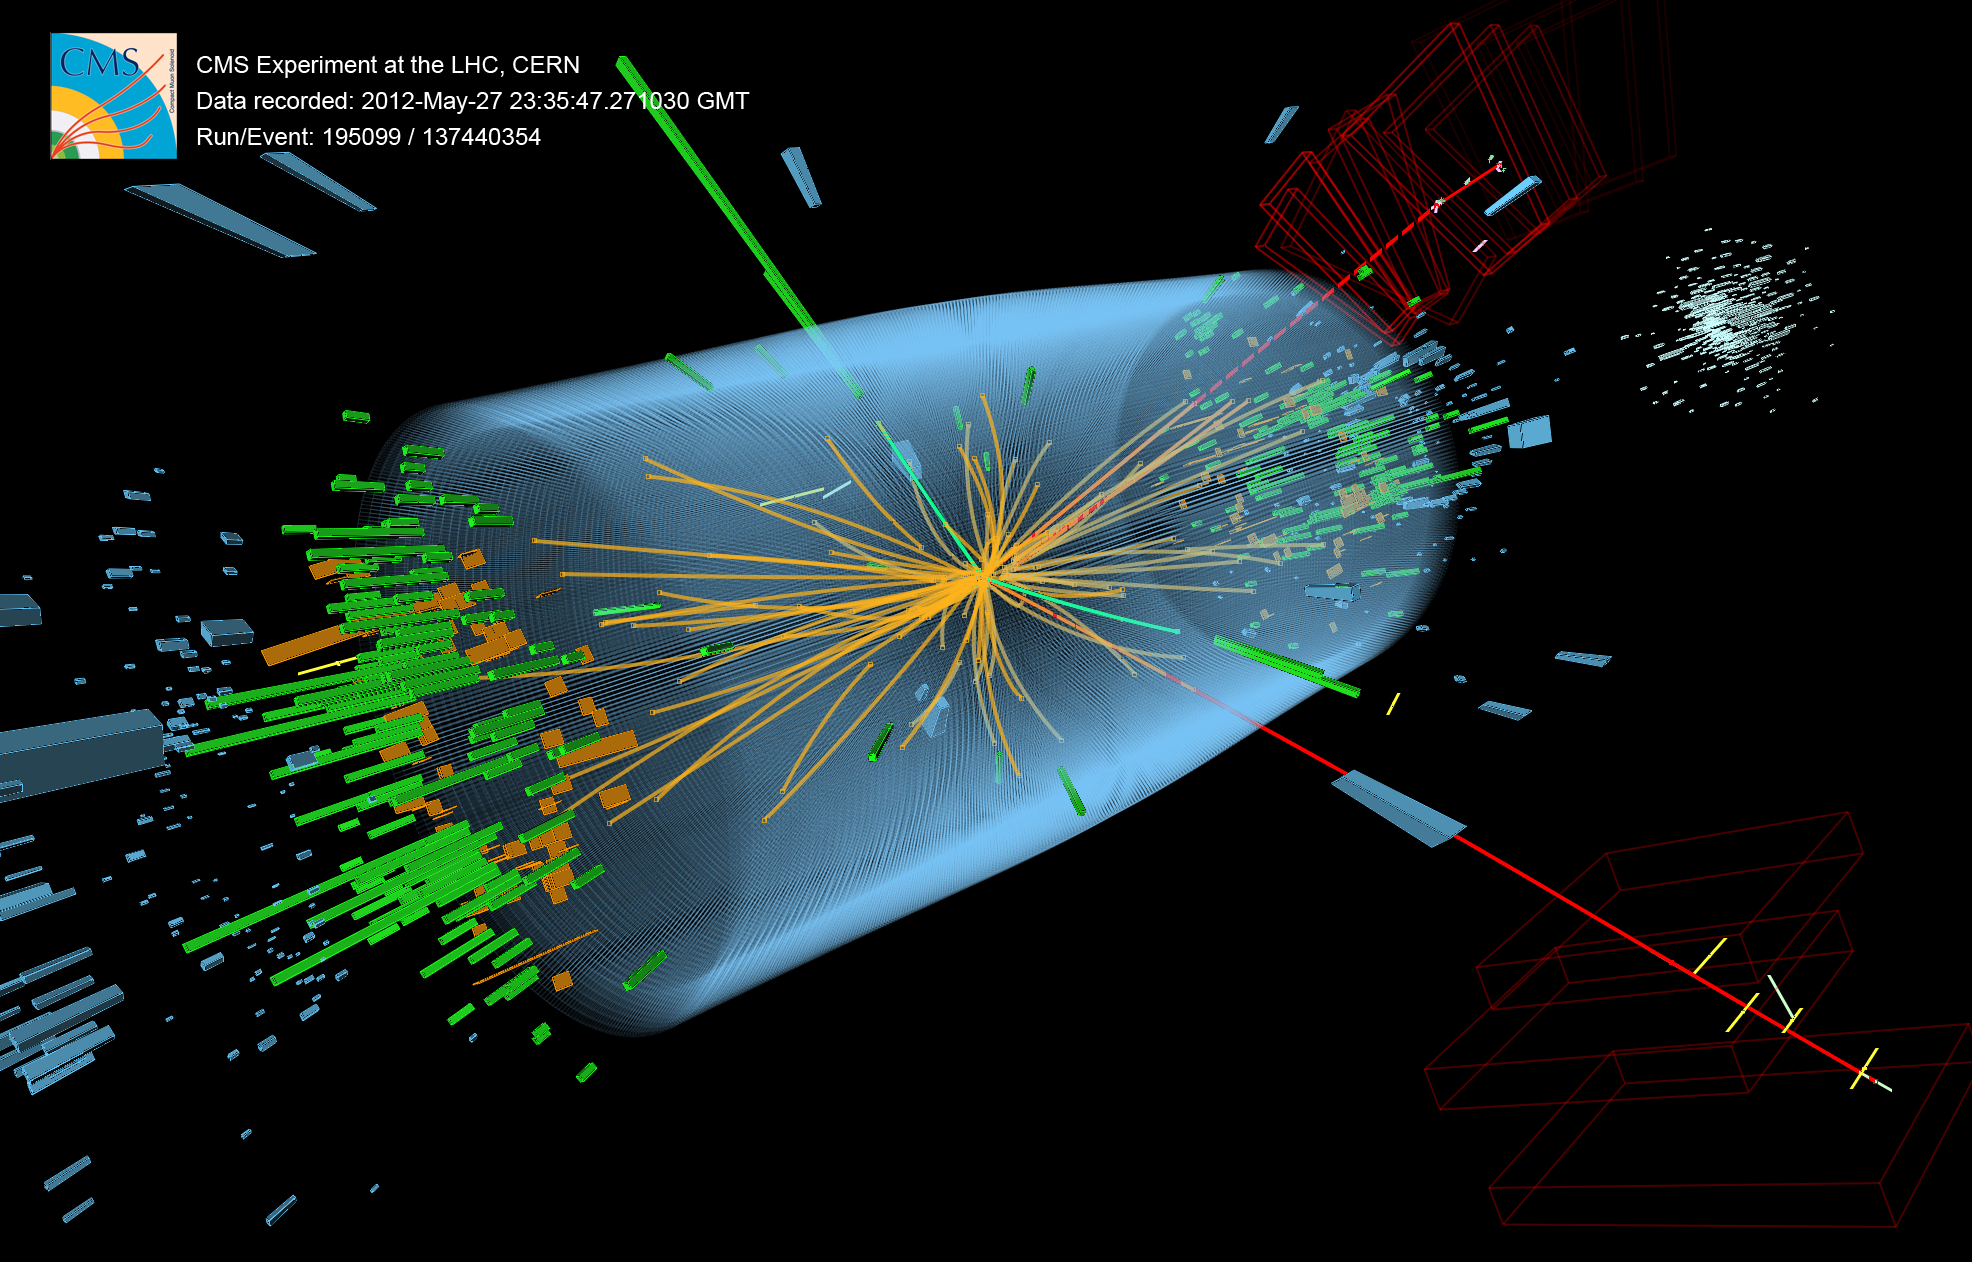
\includegraphics[width=1.00\columnwidth]{./figs/u01/higgs.png}}
  \begin{textblock*}{110mm}(10mm,0.90\textheight)
    {\bf{\alert{La física de partículas comenzó siendo física ``probabilística'' y ``colisional''}}}
  \end{textblock*}
\end{frame}

\begin{frame}
  \frametitle{``Probabilística''}
  \framesubtitle{\emph{Lo probable es lo que usualmente ocurre}, Aristóteles, Retórica, c 350 AC}
  \vspace{-0.5em}
  \begin{columns}
    \column{0.50\textwidth}
  \begin{columns}
    \column{0.50\textwidth}
    \begin{center}
      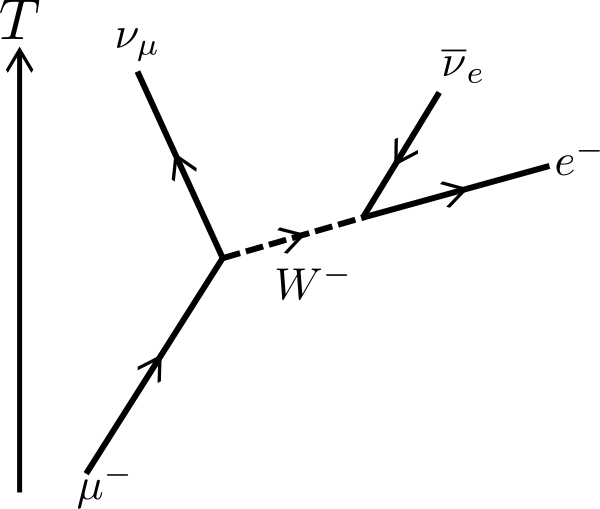
\includegraphics[width=1.0\columnwidth]{./figs/u01/muon-decay.png}
    \end{center}
    \column{0.50\textwidth}
    \vspace{+1em}
    \[ \mu^- \to e^- \bar{\nu_e} \nu_\mu \]
  \end{columns}
    \begin{itemize}
      \item Sea un muón en reposo que fue creado a $t=t_0$
      \item ¿Cuál es la probabilidad de que el muón decaiga en este instante? $\to 0$
      \item Probabilísticamente, ``instante'' no tiene sentido
      \item En $t$, la ``edad'' es $\Delta t \equiv (t-t_0)$
      \item ¿Cuál es la probabilidad de que el muón decaiga entre $\Delta t$ y $\Delta t + dt$?
      \item \alert{¿Depende de $\Delta t$?}
  \pause
    $\to$ {\Huge{\alert{¡NO!}}}
    \end{itemize}
    \column{0.50\textwidth}
    \begin{itemize}
      \item Llamemos \bblock{$\Gamma$} a la \bblock{probabilidad de decaimiento por unidad de tiempo}. 
      \item \bblock{$\Gamma$} es la \bblock{tasa de decaimiento}. 
      \item Luego, para $N_0$ muones a $t=t_0$, $dN=-\Gamma N_0 dt$, y entonces
        \be{N(t)=N_0 e^{-\Gamma t}}{EQLexp}
      \item Para un único muón, pensamos en probabilidades, la prob. de encontrar {\bf aún} al muón a tiempo $t$ es 
        \begin{alertblock}{}
          \be{P(t) = \frac1\Gamma e^{-\Gamma t} = \tau e^{-{\frac t\tau}},\ \tau\equiv\frac1\Gamma}{EQPexp}
        \end{alertblock}
      \item Y por ende, la probabilidad de decaimiento será 
        \be{P(t) = 1 - \tau e^{-{\frac t\tau}}}{EQPdec}
    \end{itemize}
  \end{columns}
\end{frame}

\begin{frame}
  \frametitle{``Probabilística''}
  \begin{columns}
    \column{0.50\textwidth}
    \begin{itemize}
      \item $\tau$ representa el tiempo de vida de las partículas,
        \vspace{-0.5em}
        \[P(t) = \tau e^{-{\frac t\tau}},\ \tau\equiv\frac1\Gamma \] 
        \vspace{-1.0em}
      \item Propiedad de falta de memoria: 
        \vspace{-0.5em}
        \[{ P[t>(\Delta t + dt) | t>\Delta t] = P[t>dt] }\]
        \vspace{-1.0em}
        \begin{itemize}
          \item Prueba: $P(A|B)=P(A\cap B)/P(B)$
          \vspace{-0.5em}
          {\tiny{
              \[ P[t>(\Delta t + dt) | t>\Delta t] = \frac{P[t>(\Delta t + dt)] \cap P[t>\Delta t] }{P[t>\Delta t]} \] 
          }}
          \vspace{-1.0em}
          \item entonces, al ser independientes y estar contenido
          \vspace{-0.5em}
          {\tiny{
          \begin{eqnarray*}
            P[t>(\Delta t + dt) | t>\Delta t] &=& \frac{P[t>(\Delta t + dt)]}{P[t>\Delta t]}\\
            P[t>(\Delta t + dt) | t>\Delta t] &=& \frac{\int_{\Delta t + dt}^\infty e^{-t/\tau} dt}{\int_{\Delta t}^\infty e^{-t/\tau} dt} \\
            P[t>(\Delta t + dt) | t>\Delta t] &=& \frac{e^{-(\Delta t + dt)/\tau}}{e^{-{\Delta t}/\tau}} \\
            P[t>(\Delta t + dt) | t>\Delta t] &=& e^{-dt/\tau} = P[t>dt]
          \end{eqnarray*}
          }}
          \vspace{-1.0em}
      \end{itemize}
    \end{itemize}
    \column{0.50\textwidth}
    \begin{itemize}
      \item Tres modos de decaimiento
      \begin{eqnarray*}
        \mu^- \to e^- \bar{\nu_e} \nu_\mu         &\quad& \approx 100\%\\
        \mu^- \to e^- \bar{\nu_e} \nu_\mu \gamma  &\quad& 1.4\times10^{-2}\\
        \mu^- \to e^- \bar{\nu_e} \nu_\mu e^+ e^- &\quad& 3.4\times10^{-5}
      \end{eqnarray*}
      \item Como siempre, a priori no podremos determinar, cuál seguirá, y con que probabilidad (lo haremos)
      \item Cada modo, tendrá su propia \bblock{tasa de decaimiento $\Gamma_i$}:
        \be{\Gamma_{\mathrm{tot}} = \sum_{i=1}^N \Gamma_i,\ \tau = \frac 1 \Gamma_{\mathrm{tot}} }{EQDecayRate}
      \item Con esto, queda definido el
      \bc{{\bf{\alert{\emph{Branching ratio}}} $\equiv \Gamma_i / \Gamma_{\mathrm{tot}}$.}}
      \vspace{-0em}
      \[ \mu^- \to e^- \bar{\nu_e} \nu_\mu,\quad \Gamma_i / \Gamma_{\mathrm{tot}} \approx 100\% \]
    \end{itemize}
  \end{columns}
\end{frame}
\end{document}
